\chapter{Messung der Streuspektren}

\section{Theoretische Grundlagen}

Aus der relativistischen Compton-Formel (Gl.~\ref{eq:compton}) folgt, dass sich der Vollenergiepeak des Primärstrahls mit zunehmendem Streuwinkel zu kleineren Energien verschiebt. 
Gleichzeitig entsteht durch die Streuung der Photonen an Elektronen ein kontinuierliches Energiespektrum, das sogenannte Compton-Kontinuum. 
Das gemessene Spektrum enthält somit sowohl den Vollenergiepeak als auch das Compton-Kontinuum, dessen Energiebereich sich von der Energie des Primärphotons bis zum Compton-Edge erstreckt.

Durch die Aufnahme der Spektren für verschiedene Streuwinkel $\theta$ kann die Winkelabhängigkeit der Energie der gestreuten Photonen experimentell untersucht werden.

Die Energie des gestreuten Photons ergibt sich aus

\begin{align}
    E_{\gamma'}(\theta)
    =
    \frac{E_\gamma}
    {1+\frac{E_\gamma}{m_ec^2}(1-\cos\theta)}
    \label{eq:compton_fit}
\end{align}

mit der Photonenergie $E_\gamma$ des Primärstrahls und dem Streuwinkel $\theta$.

Neben der Energieverteilung ist auch die Winkelabhängigkeit der Streuintensität von Interesse. 
Zusätzlich lässt sich aus der Winkelabhängigkeit der Streuintensität mithilfe der Klein-Nishina-Formel \cite{KleinNishina1929} der differentielle Wirkungsquerschnitt der Compton-Streuung bestimmen:

\begin{align}
    \frac{d\sigma}{d\Omega} = \frac{r_e^2}{2} \left( \frac{E_{\gamma'}}{E_{\gamma}} \right)^2 \left( \frac{E_{\gamma'}}{E_{\gamma}} + \frac{E_{\gamma}}{E_{\gamma'}} - \sin^2 \theta \right)
    \label{form:KleinNishima}
\end{align}

Hierbei bezeichnet $r_e$ den klassischen Elektronenradius.

\section{Durchführung}

Zur Erzeugung eines definierten Einzelstreuprozesses, wurde eine $1\,\mathrm{mm}$ dicke Aluminiumfolie auf den kollimierten Gammastrahl gelegt. 
Die gestreuten Photonen wurden in $5^\circ$-Schritten unter einem Winkel von $35^\circ$  bis $120^\circ$ detektiert. 

Für diese Messung wurde ein $3\,\mathrm{cm}$ großer Kollimator verwendet, um eine hohe Messgeschwindigkeit zu gewährleisten. 
Da die Streueffizienz einzelner Teilchen im Target geringer ist, erhöht ein größerer Kollimator die Empfindlichkeit des Detektors, ohne die Winkelauflösung wesentlich zu beeinträchtigen.

\paragraph{Untergrundmessung}

Auch ohne eingesetztes Streutarget werden Photonen im Detektor registriert. 
Diese Beiträge entstehen unter anderem durch Streuung an Bleiteilen des Aufbaus, an Luftmolekülen oder direkt am Detektormaterial.

Da dieser Untergrund winkelabhängig ist, wurde für jede Detektorposition eine separate Hintergrundmessung ohne Aluminiumtarget durchgeführt. 
Die Messdauer betrug sowohl für die Untergrund- als auch für die Streumessung jeweils $300\,\mathrm{s}$.

Das reine Streusignal ergibt sich aus der Differenz

\begin{align}
    N_\mathrm{Streu}(\theta)
    =
    N_\mathrm{mit\ Target}(\theta)
    -
    N_\mathrm{ohne\ Target}(\theta).
\end{align}

\section{Auswertung}

Nun soll die Abhängigkeit der gestreuten Photonenenergie vom Winkel untersucht werden, und den entsprechenden Wirkungsquerschnitt mit Hilfe der Klein-Nishima-Formel (Gl.\ref{form:KleinNishima}) für die Compton-Streuung zu bestimmt werden.

\subsection{Überprüfung der Compton-Beziehung}

Zunächst wurde die Winkelabhängigkeit der Energie der gestreuten Photonen untersucht. 
Hierzu wurden die Photopeaks der einzelnen Spektren mithilfe von Gaußfunktionen angepasst. 
Die Peakpositionen in Kanalnummern sind in Tabelle~\ref{tab:gauss_intensities} aufgeführt. 
Anschließend wurden diese mithilfe der zuvor bestimmten Energiekalibrierung in Photonenergien umgerechnet.

Die theoretische Beschreibung der Winkelabhängigkeit erfolgt durch die Compton-Formel Gl.\ref{eq:compton_fit} wobei $E_\gamma$ die Energie des Primärphotons bezeichnet.

Die Ergebnisse der Anpassung sind in Abb.~\ref{plot:Compton} dargestellt. 
Aus dem Fit ergibt sich eine Primärenergie von

\begin{align}
    E_\gamma
    =
    (637,9 \pm 7,4)\,\mathrm{keV}.
\end{align}

Dieser Wert stimmt innerhalb einer $3\sigma$-Abweichung mit der Literaturenergie von $661{,}7\,\mathrm{keV}$ des $^{137}$Cs-Zerfalls überein \cite{nndc_152eu_decaydata}.

Der reduzierte $\chi^2$-Wert von

\begin{align}
    \chi^2_\mathrm{red}=0,08
\end{align}

zeigt eine sehr gute Übereinstimmung zwischen den Messdaten und dem theoretischen Modell.

\begin{figure}[htbp]
    \centering
    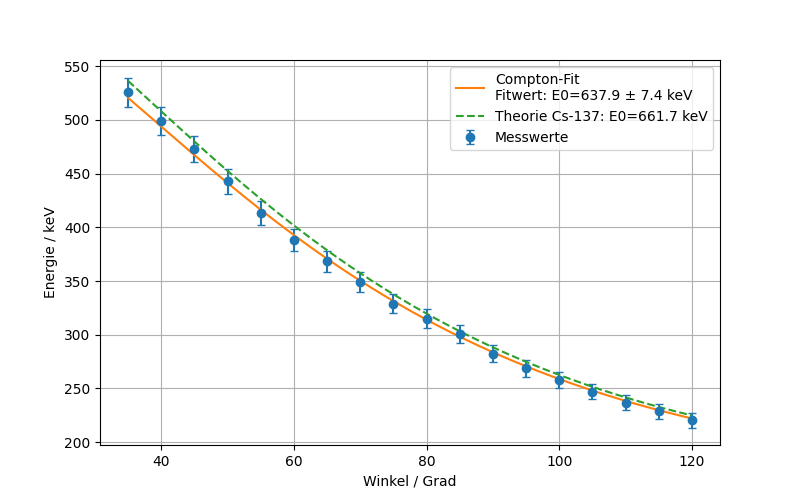
\includegraphics[width=0.75\textwidth]{figs/Comptenfianlefertg.png}
    \caption{Energie der gestreuten Photonen in Abhängigkeit vom Streuwinkel.}
    \label{plot:Compton}
\end{figure}

\FloatBarrier

Wie zu erwarten, nimmt die Intensität des Vollenergiepeaks mit dem zunehmendem Streuwinkel ab. 
Insbesondere bei größeren Streuwinkeln wird der Vollenergiepeak deutlich abgeschwächt, da mehr Photonen Energie an die Elektronen abgeben und somit im Compton-Kontinuum landen.

\begin{table}[htbp]
\centering
\caption{Intensitäten und Peakparameter aus Gaußfits für verschiedene Streuwinkel.}
\begin{tabular}{cccccccc}
\hline
$\theta/^\circ$ & Kanal & $\Delta$Kanal & $E$/keV & $\Delta E$/keV & Intensität & $\Delta I$ & $\chi^2_\mathrm{red}$ \\
\hline
35  & 5359,87 & 6,16  & 525,77 & 13,62 & 9438,35 & 97,15 & 1,74 \\
40  & 5088,21 & 6,67  & 498,51 & 12,98 & 8401,19 & 91,66 & 1,77 \\
45  & 4833,39 & 6,36  & 472,94 & 12,38 & 7681,06 & 87,64 & 1,36 \\
50  & 4534,87 & 7,01  & 442,98 & 11,68 & 7315,08 & 85,53 & 1,75 \\
55  & 4236,85 & 6,87  & 413,08 & 10,98 & 7199,38 & 84,85 & 1,53 \\
60  & 3989,51 & 9,13  & 388,26 & 10,42 & 6791,52 & 82,41 & 2,00 \\
65  & 3789,90 & 7,94  & 368,23 & 9,95  & 6787,18 & 82,38 & 2,16 \\
70  & 3597,93 & 8,18  & 348,96 & 9,51  & 6638,29 & 81,48 & 2,10 \\
75  & 3397,56 & 10,64 & 328,86 & 9,08  & 6444,47 & 80,28 & 2,34 \\
80  & 3260,46 & 14,29 & 315,10 & 8,83  & 6365,49 & 79,78 & 2,64 \\
85  & 3118,11 & 10,45 & 300,82 & 8,46  & 5942,04 & 77,08 & 3,68 \\
90  & 2935,33 & 9,78  & 282,48 & 8,04  & 6525,06 & 80,78 & 3,30 \\
95  & 2798,83 & 10,35 & 268,78 & 7,75  & 6155,77 & 78,46 & 4,30 \\
100 & 2689,33 & 9,62  & 257,79 & 7,50  & 6470,45 & 80,44 & 3,99 \\
105 & 2582,65 & 10,09 & 247,09 & 7,28  & 6829,45 & 82,64 & 4,09 \\
110 & 2480,77 & 7,40  & 236,86 & 7,03  & 7169,22 & 84,67 & 3,71 \\
115 & 2398,77 & 5,18  & 228,63 & 6,83  & 6663,25 & 81,63 & 4,70 \\
120 & 2316,13 & 6,86  & 220,34 & 6,67  & 7059,46 & 84,02 & 5,49 \\
\hline
\end{tabular}
\label{tab:gauss_intensities}
\end{table}

Die mithilfe der Energiekalibrierung bestimmten Photonenergien sind in Tabelle~\ref{tab:gauss_intensities} aufgeführt. 
Die gemessene Winkelabhängigkeit der gestreuten Photonenergie wurde anschließend mithilfe der Compton-Formel aus Gl.~\ref{eq:compton_fit} beschrieben, wobei die Energie des Primärphotons $E_\gamma$ als freier Fitparameter verwendet wurde.

Abbildung~\ref{plot:Compton} zeigt die Energie der gestreuten Photonen $E_{\gamma'}$ in Abhängigkeit vom Streuwinkel $\theta$. 
Die theoretische Anpassung beschreibt die Messdaten insgesamt gut und bestätigt die erwartete Winkelabhängigkeit der Compton-Streuung.

Die verbleibenden Abweichungen zwischen Messdaten und Fit lassen sich auf experimentelle Unsicherheiten zurückführen, beispielsweise auf statistische Schwankungen, Unsicherheiten der Energiekalibrierung oder Fehler bei der Winkelbestimmung.

Insgesamt zeigt die gute Übereinstimmung zwischen Theorie und Messung, dass die Compton-Formel die Energie gestreuter Photonen in Abhängigkeit vom Streuwinkel adäquat beschreibt.

\subsection{Winkelabhängigkeit der Streuintensität}

Zur Untersuchung der Winkelabhängigkeit der Streuintensität wurden die gemessenen Intensitäten auf den Wert bei $\theta=35^\circ$ normiert. 
Zusätzlich wurde eine Effizienzkorrektur durchgeführt, um die energieabhängige Nachweiswahrscheinlichkeit des Detektors zu berücksichtigen.

Die normierten Intensitäten sind in Abb.~\ref{plot:nk-plot} dargestellt.

\begin{figure}[htbp]
    \centering
    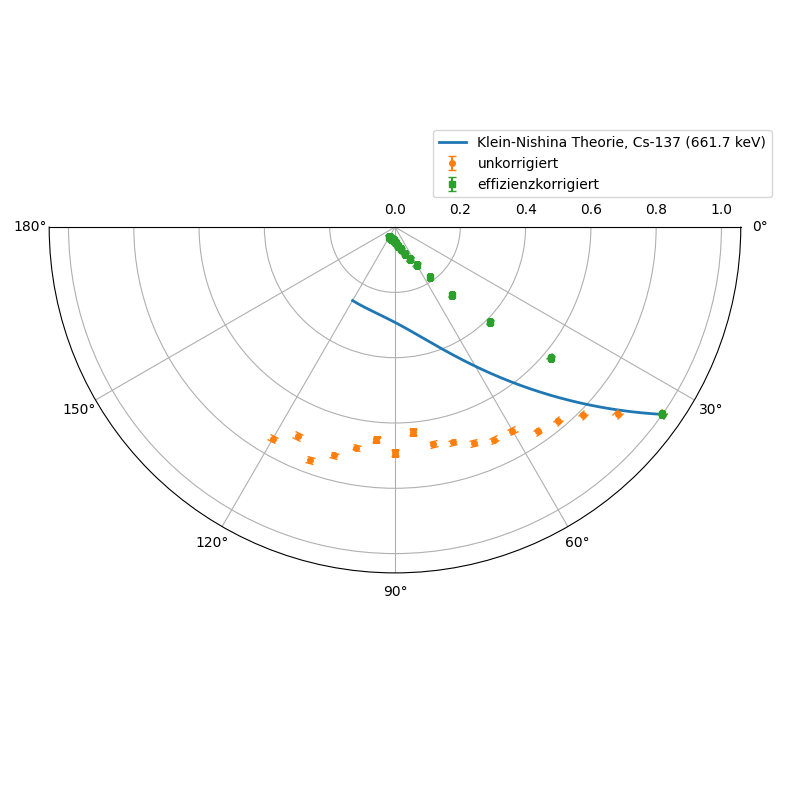
\includegraphics[width=0.75\textwidth]{figs/kn-plot-fertig.png}
    \caption{Normierte Streuintensität in Abhängigkeit vom Streuwinkel.}
    \label{plot:nk-plot}
\end{figure}

\FloatBarrier

Die unkorrigierten Messwerte zeigen insgesamt eine Abnahme der Intensität mit wachsendem Streuwinkel. 
Besonders im Bereich um $\theta=90^\circ$ tritt ein deutliches Intensitätsminimum auf.

Eine mögliche Ursache hierfür ist die veränderte effektive Weglänge der Photonen im Aluminiumtarget. 
Je nach Streuwinkel verändert sich die Strecke, die das gestreute Photon innerhalb des Materials zurücklegen muss. 
Dadurch steigt die Wahrscheinlichkeit zusätzlicher Absorption oder Mehrfachstreuung.

Nach Anwendung der Effizienzkorrektur fällt die Intensität bei großen Winkeln deutlich stärker ab. 
Dies hängt damit zusammen, dass die Energie der gestreuten Photonen mit wachsendem Winkel kleiner wird. 
Da die Detektoreffizienz energieabhängig ist, wirken sich kleine Unsicherheiten der Effizienzkorrektur bei niedrigen Energien besonders stark aus.

\begin{table}[htbp]
\centering
\caption{Normierte Intensitäten in Abhängigkeit des Streuwinkels.}
\begin{tabular}{ccccc}
\hline
$\theta/^\circ$ &
$I_{\mathrm{raw,norm}}$ &
$\Delta I_{\mathrm{raw,norm}}$ &
$I_{\mathrm{corr,norm}}$ &
$\Delta I_{\mathrm{corr,norm}}$ \\
\hline
35  & 1,00000 & 0,01029 & 1,00000 & 0,01029 \\
40  & 0,89011 & 0,00971 & 0,62244 & 0,00679 \\
45  & 0,81381 & 0,00929 & 0,41070 & 0,00469 \\
50  & 0,77504 & 0,00906 & 0,27037 & 0,00316 \\
55  & 0,76278 & 0,00899 & 0,18696 & 0,00220 \\
60  & 0,71957 & 0,00873 & 0,13337 & 0,00162 \\
65  & 0,71911 & 0,00873 & 0,10745 & 0,00130 \\
70  & 0,70333 & 0,00863 & 0,08624 & 0,00106 \\
75  & 0,68280 & 0,00851 & 0,06886 & 0,00086 \\
80  & 0,67443 & 0,00845 & 0,05994 & 0,00075 \\
85  & 0,62956 & 0,00817 & 0,04940 & 0,00064 \\
90  & 0,69133 & 0,00856 & 0,04674 & 0,00058 \\
95  & 0,65221 & 0,00831 & 0,03982 & 0,00051 \\
100 & 0,68555 & 0,00852 & 0,03880 & 0,00048 \\
105 & 0,72359 & 0,00876 & 0,03826 & 0,00046 \\
110 & 0,75958 & 0,00897 & 0,03786 & 0,00045 \\
115 & 0,70598 & 0,00865 & 0,03370 & 0,00041 \\
120 & 0,74796 & 0,00890 & 0,03433 & 0,00041 \\
\hline
\end{tabular}
\label{tab:winkel_intensitaet}
\end{table}

Für eine präzisere Untersuchung der Winkelabhängigkeit wären längere Messzeiten sowie eine genauere Bestimmung der Detektoreffizienz erforderlich. 
Insbesondere bei großen Streuwinkeln führen kleine statistische Unsicherheiten aufgrund der niedrigen Intensitäten zu vergleichsweise großen relativen Fehlern.
